\documentclass[letterpaper,12pt,fullpage]{article}

\usepackage[left=1in,right=1in,top=1in,bottom=1in]{geometry}
% \usepackage{cite}
\usepackage{graphicx}
% \usepackage[dvips]{graphicx}
% \usepackage{epsfig} % for postscript graphics files
  % \graphicspath{{../eps/}}
% \DeclareGraphicsExtensions{.eps}
\usepackage{amsmath}
\usepackage{amssymb}
%\usepackage[cmex10]{amsmath}
%\usepackage{array}
%\usepackage{mdwmath}
%\usepackage{mdwtab}
%\usepackage{eqparbox}
\usepackage[tight,footnotesize]{subfigure}
%\usepackage[caption=false]{caption}
%\usepackage[font=footnotesize]{subfig}
%\usepackage{fixltx2e}
%\usepackage{stfloats}
\usepackage{hyperref}
\usepackage[backend=biber]{biblatex}
\addbibresource{exos/bleex.bib}
\addbibresource{exos/hal.bib}
\addbibresource{exos/xor.bib}


% correct bad hyphenation here
%\hyphenation{op-tical net-works semi-conduc-tor}
% for LaTeX

% Single and double spacing. {\single text} or {\double text}
\newcommand{\single}{\def\baselinestretch{1.0}\large\normalsize}
\newcommand{\double}{\def\baselinestretch{1.5}\large\normalsize}
\newcommand{\triple}{\def\baselinestretch{2.0}\large\normalsize}

\def \tilde{\raisebox{-0.7 ex}{\char`\~}}
% or $\sim$

% Margin notes. \note{note to myself.}
%\newcommand{\note}[1]{\marginpar{\raggedright \small [#1]}}

% BibTex fix so \"{o} does not screw things up.
\newcommand{\dd}[1]{{\"{#1}}}

% Abbreviations for greek letters
\newcommand{\al}{{\alpha}}
\newcommand{\ep}{{\epsilon}}
\newcommand{\la}{{\lambda}}
\newcommand{\ga}{{\gamma}}
\newcommand{\om}{{\omega}}

% vectors
\newcommand{\va}{{\bf a}}
\newcommand{\vb}{{\bf b}}
\newcommand{\vc}{{\bf c}}
\newcommand{\ve}{{\bf e}}
\newcommand{\vf}{{\bf f}}
\newcommand{\vg}{{\bf g}}
\newcommand{\vh}{{\bf h}}
\newcommand{\vi}{{\bf i}}
\newcommand{\vk}{{\bf k}}
\newcommand{\vl}{{\bf l}}
\newcommand{\vm}{{\bf m}}
\newcommand{\vn}{{\bf n}}
\newcommand{\vp}{{\bf p}}
\newcommand{\vq}{{\bf q}}
\newcommand{\vr}{{\bf r}}
\newcommand{\vs}{{\bf s}}
\newcommand{\vt}{{\bf t}}
\newcommand{\vu}{{\bf u}}
\newcommand{\vv}{{\bf v}}
\newcommand{\vw}{{\bf w}}
\newcommand{\vx}{{\bf x}}
\newcommand{\vy}{{\bf y}}
\newcommand{\vz}{{\bf z}}

% Greek vectors
% We get bold greek letters from:
%\font\boldmathitalic=ambi10 at 12pt

%\newcommand{\vomega}{\hbox{\boldmathitalic !}}
%\newcommand{\vphi}{\hbox{\boldmathitalic \char'036}}
%\newcommand{\vpsi}{\hbox{\boldmathitalic \char'040}}
%\newcommand{\vtau}{\hbox{\boldmathitalic \char'034}}
%\newcommand{\vtheta}{{\bf \theta}}

% bkph's bold greek letter hack.
\def\boldify#1{\hbox{\rlap{$#1$}\kern .4pt{$#1$}}} % attempt bold Greek letter
% not needed for upper case Greek, which does come in bold! 0.6pt ?

\newcommand{\valpha}{\boldify{\alpha}}
\newcommand{\vepsilon}{\boldify{\epsilon}}
\newcommand{\vomega}{\boldify{\omega}}
\newcommand{\vpi}{\boldify{\pi}}
\newcommand{\vphi}{\boldify{\phi}}
\newcommand{\vpsi}{\boldify{\psi}}
\newcommand{\vtau}{\boldify{\tau}}
\newcommand{\vtheta}{\boldify{\theta}}

% doesn't look bold to me
% The bm package, which is part of the LaTeX tools distribution,
% defines a command \bm which may be used anywhere in maths mode. 
% \newcommand{\vpi}{{\bm \pi}}

% did not work
% this should be \boldmath \unboldmath p. 53, 201 
% \newcommand{\valpha}{{\mbox{\boldmath $\alpha$}}}

% did not work
% \newcommand{\vpi}{{\mbox{\bf $\pi$}}}

\newcommand{\vep}{{\vepsilon}}
\newcommand{\vom}{\vomega}
\newcommand{\vph}{\vphi}
\newcommand{\vps}{\vpsi}
\newcommand{\vta}{\vtau}
\newcommand{\vth}{\vtheta}

% matrices
\newcommand{\mA}{{\bf A}}
\newcommand{\mB}{{\bf B}}
\newcommand{\mC}{{\bf C}}
\newcommand{\mD}{{\bf D}}
\newcommand{\mE}{{\bf E}}
\newcommand{\mF}{{\bf F}}
\newcommand{\mG}{{\bf G}}
\newcommand{\mH}{{\bf H}}
\newcommand{\mI}{{\bf I}}
\newcommand{\mJ}{{\bf J}}
\newcommand{\mK}{{\bf K}}
\newcommand{\mL}{{\bf L}}
\newcommand{\mM}{{\bf M}}
\newcommand{\mP}{{\bf P}}
\newcommand{\mQ}{{\bf Q}}
\newcommand{\mR}{{\bf R}}
\newcommand{\mS}{{\bf S}}
\newcommand{\mT}{{\bf T}}
\newcommand{\mU}{{\bf U}}
\newcommand{\mV}{{\bf V}}
\newcommand{\mW}{{\bf W}}
\newcommand{\mX}{{\bf X}}
\newcommand{\mZ}{{\bf Z}}

\newcommand{\mOmega}{{\bf \Omega}}
\newcommand{\mPi}{{\bf \Pi}}

\newcommand{\mSigma}{\hbox{\bf \char'006}}

\newcommand{\Ep}{{E}}

\newcommand{\id}{{\bf 1}}

% transpose
\newcommand{\tr}{{\rm T}}

% probability
\newcommand{\prob}{{\mbox p}}

% variance
\newcommand{\var}{{\mbox {Var}}}

% trace
\newcommand{\trace}{{\mbox {trace}}}

% expectation
\newcommand{\E}{{\mbox {E}}}

% and, or
\newcommand{\aand}{{\mbox {and}}}
\newcommand{\oor}{{\mbox {or}}}

% argmin
%\newcommand{\argmin}{{\mbox {argmin}}}

% time handling (stolen from YTEX)
\newcount\hour
\newcount\minute
\hour=\the\time \minute=\the\time
\divide\hour by 60 \multiply\hour by 60%
\advance\minute by -\hour \divide\hour by 60%
\newcommand{\thetime}{\number\hour:\ifnum \minute<10 0\fi\number\minute}%

\newcommand{\mypsfig}[2]{\centerline{\psfig{file=#1,height=#2}}}
\newcommand{\vwhat}{\widehat{\vw}}


\begin{document}

\title{A Survey of Exoskeleton Control Architectures and
Algorithms\\
(Draft 3.0)}

\author{Alex Ansari, Christopher G. Atkeson, Howie Choset, and Matthew Travers\\
Carnegie Mellon University}

\maketitle

\begin{abstract}
Abstract to be written.
\end{abstract}

\section{Executive Summary}

Executive Summary to be written.

\section{Scope: What is this paper about?}

This paper surveys exoskeleton control architectures and
algorithms.
The focus is on exoskeleton control that allows a
highly trained and top percentile athletic 
operator to carry a payload that weighs approximately the same amount
as the operator. We envisage these types of exoskeletons to be useful
in carrying protective and safety equipment for SWAT teams, police,
firefighters, and soldiers. 
We also 
focus this survey on exoskeleton control for lower body tasks (standing, walking,
running, jumping, kicking, dodging, ...).

\section{BLEEX}
\label{exo:bleex}

keywords: sensitivity amplification; strength augmentation.\\

The Berkeley lower extremity exoskeleton (BLEEX) is an anthropomorphic, powered exoskeleton designed for human strength augmentation.  It is described as the first field-operational robotic system to allow its operator to carry significant loads over unstructured terrain without external power \cite{bleex_design_2006}.

\begin{figure}[ht]
  \centering
  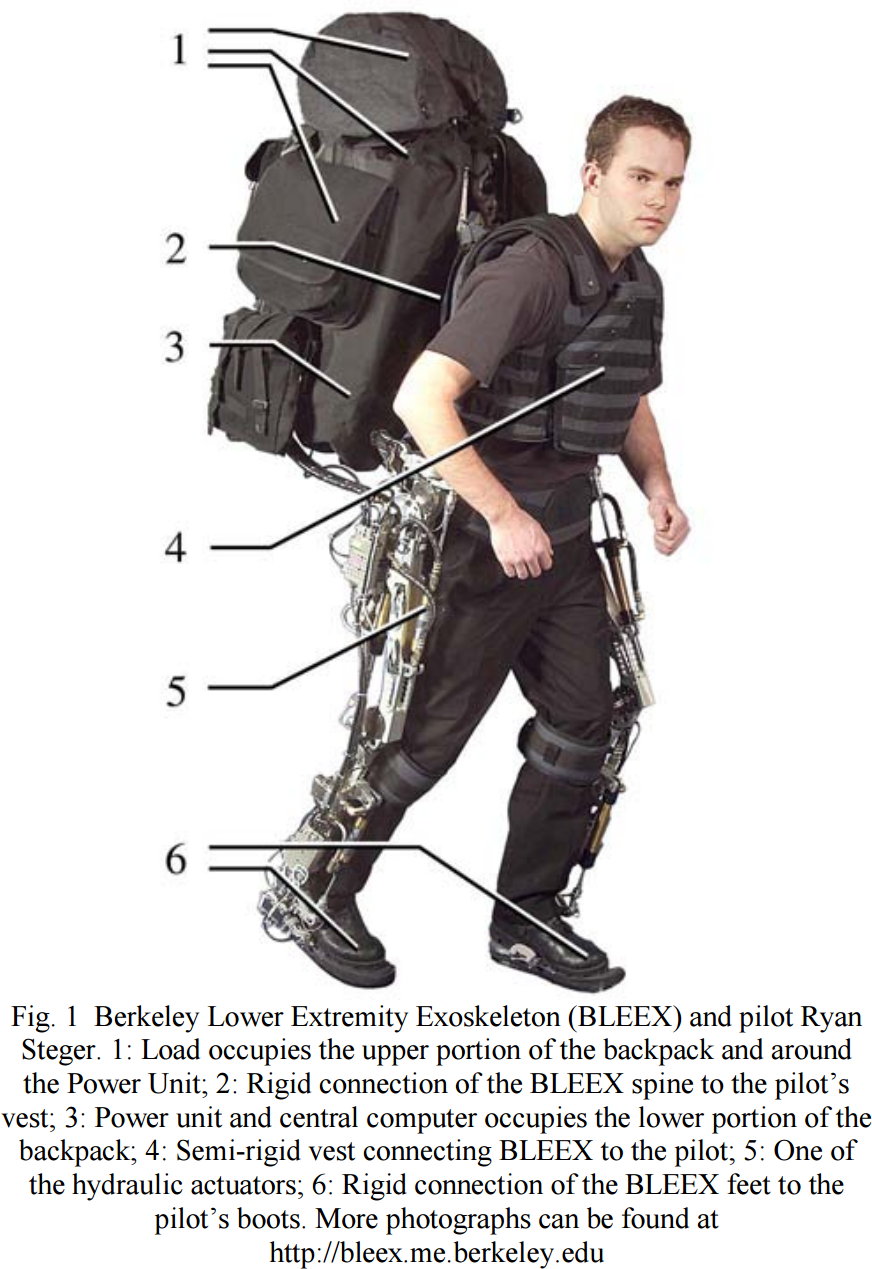
\includegraphics[width=3.5in]{exos/figs/bleex_exo.png}
\end{figure}

The BLEEX system includes two 7 DOF, three-segment legs with thigh, shank, and foot links, on-board power supply, and a backpack-like frame.  The human wearer is rigidly connected at the feet and torso such that the frame shelters the user by transferring load forces to the ground.  The leg segments are connected by rotational joints including 3 DOF (2 actuated) at the hip, 1 DOF (actuated) at each knee, and 3 DOF (1 actuated f/e in sagittal 
plane; 2 passive) at the ankles.  Joint angles, torque, and power requirements are determined from human motion analysis based on a 75-kg human walking on flat ground at roughly 1.3 m/s (the average military male's maximum reported joint limits are also used to derive joint range of motion targets).  During design, joint motion was intended to be slightly less than the maximum human range of motion for safety; however, some joint ranges had to be reduced to avoid singularities.
% Ideally, joint motion would provide the maximum human range of motion for safety

Due to its high power to weight ratio (twice that of electric motors), BLEEX uses a hydraulic actuation system.  An on-board internal combustion engine provides both electric and hydraulic power.  The joints are driven by commercial small bore (2cm) dual action hydraulic actuators operating at 6.9 MPa. Though the operating pressure is relatively low, the hydraulic actuation system exhibits significant pressures losses across servo valves when less pressure is required than this system pressure.  Table~\ref{tab:bleex_joints} provides details regarding the range of motion and torque capabilities of BLEEX's joints.  As reported in \cite{bleex_design_2006}, BLEEX requires 1,143 W for walking relative to 165 W for human walking (14\% efficient compared to a human of the same size).  Altogether the suit needs 2.27 kW of hydraulic power and 220 W of electric power to accommodate climbing (540 W) and remaining electrical loads including 240 W to power the second stages on servo vales.

%
\begin{table}
\centering
\begin{tabular}{|l|*{3}{c|}}  % repeats {c|} 6 times
\hline
& BLEEX & human max & BLEEX \\
& ROM & torque \& power & max torque \\ \hline
Ankle flexion / extension & $\pm 45^\circ$ & $-120$ N-m; 250 W & $-200 / 155$ N-m\\ \hline
Ankle abduction / adduction & $\pm 20^\circ$ & N/A & N/A \\ \hline
Knee flexion & $121^\circ$ & $-35 / 60$ N-m; $-150 / 50$ W & $-100 / 140$ N-m \\ \hline
Hip flexion / extension & $\pm 121^\circ / 10^\circ$ & $-80 / 60$ N-m; $-60 / 115$ W & $-150 / 130$ N-m \\ \hline
Hip abduction / adduction & $\pm 16^\circ$ & N/A & N/A\\ \hline
total rotation external & $35^\circ$ & N/A & N/A \\ \hline
total rotation internal & $35^\circ$ & N/A & N/A \\ \hline
\end{tabular}
\caption{BLEEX joint range of motion (ROM) is near anthropomorphic.  The max torques are designed to meet the torque / power requirements of similarly sized human walking at 1.3 m/s \cite{bleex_design_2006}.}\label{tab:bleex_joints}
\end{table}
%

\subsubsection{Control}

The BLEEX team has successfully implemented both sensitivity amplification \cite{sesitivityAmpPaper2005} and a hybrid assitive control scheme \cite{bleex_hybrid_control_2006} that switches (based on gait phase) between sensitivity amplification and a position control regulating desired torque. This section focuses on sensitivity amplification, as the hybrid assitive strategy did not perform as well in walking trials.

\begin{figure}[ht]
  \centering
  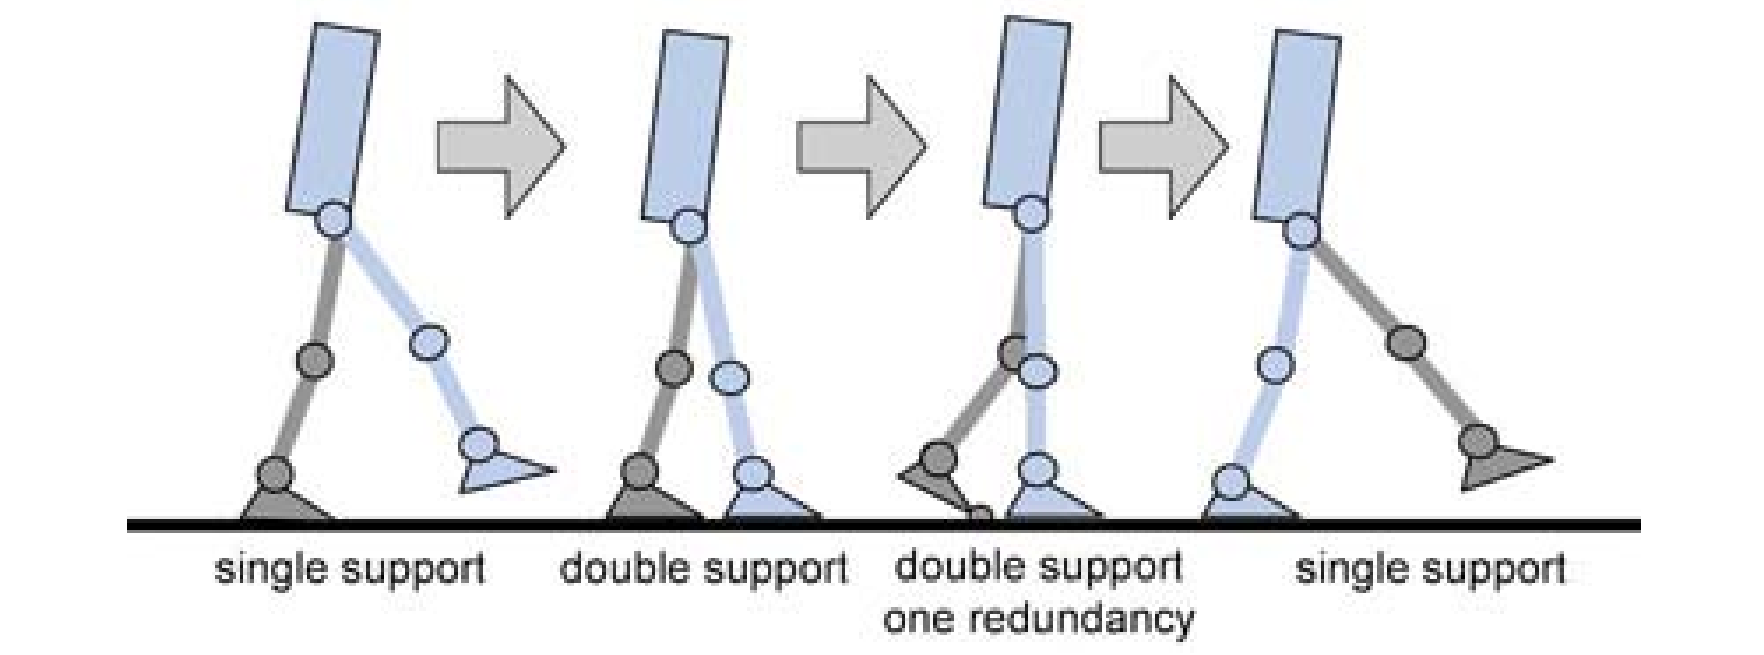
\includegraphics[width=3.5in]{exos/figs/bleex_support_phases.png}
\end{figure}

In its sensitivity amplification implementation, BLEEX controllers attempt to minimize interaction forces between the human pilot and the exoskeleton. However, the BLEEX team makes a point to avoid direct measurements of the interaction force between the human and the exoskeleton suit.  They highlight difficulties in properly outfitting humans with necessary sensing equipment and challenges in modeling the interaction between the human and exoskeleton (e.g., non-rigid, non-fixed contact points).  Instead, the team develops controllers based on an inverse dynamic model (in the saggital plane) of only the exoskeleton.  

\begin{figure}[ht]
  \centering
  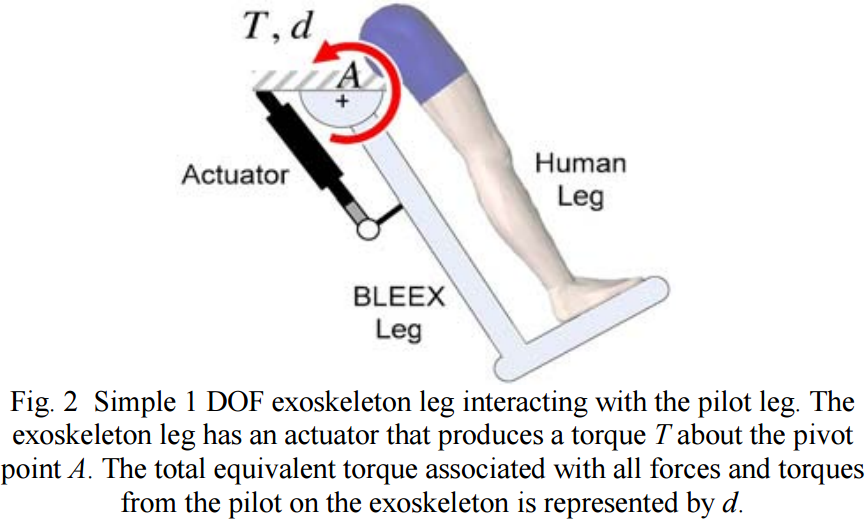
\includegraphics[width=3.5in]{exos/figs/bleex_1dof_ex.png}
\end{figure}

Assuming no outside disturbances, the BLEEX sensitivity amplification control strategy models the torque applied by the human pilot on the exoskeleton as $d$ (assuming no outside disturbances).   Neglecting gravity, the exokeleton angular velocity is modeled as 
\[v = G r + S d ,\] 
where $v$ represents the angular velocity of the exokeleton, $G$ is the transfer function from actuator inputs ($G$ is the exoskeleton's dynamics), $r$ is the actuator input, and $S$ is the sensitivity or transfer function from human torque to exokeleton angular velocity. 

\begin{figure}[ht]
  \centering
  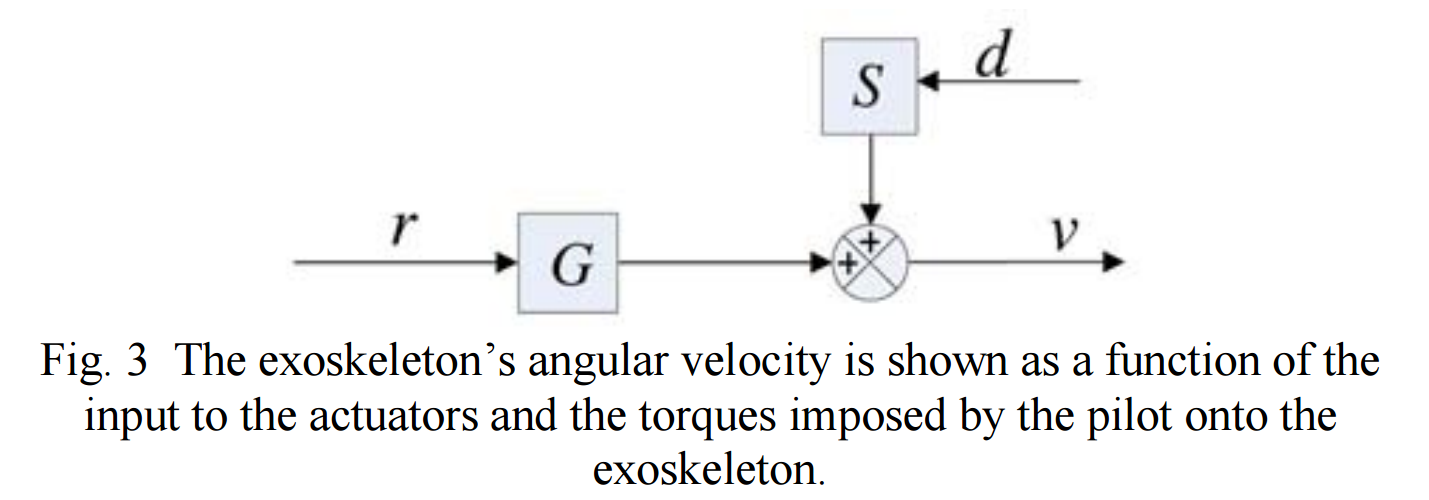
\includegraphics[width=4.0in]{exos/figs/bleex_control_diag_1.png}
\end{figure}

The goal is to maximize sensitivity to $d$ \emph{without direct measurement.}  Sensitivity amplification accomplishes this by creating a feedback loop from a controller, $C$, acting only on exoskeleton variables.  A new sensitivity equation,
\[S_{new} = \frac{v}{d} = \frac{S}{1 + G C} ,\]
is maximized by applying positive feedback.  To achieve a large sensitivity, BLEEX uses $C = (1-\alpha^{-1})G^{-1}$ so that $\alpha$ provides a direct (scalar) amplification factor. A low pass filter is often added to the $C$ term in order to damp out high frequency dynamics of the exoskeleton, which are not captured in these models.  Note that the controller depends on an inverse dynamic model of the exoskeleton, $G^{-1}$.  Since the model is hybrid, these dynamics switch according to gait phases (single support, double support, stance).  BLEEX detects these transitions using foot sensors.  Assuming the single leg support dynamics are in the form,
\begin{equation}
\mM({\bf\theta})\ddot{{\bf \theta}} + \mC({\bf\theta},\dot{{\bf\theta}}) \dot{{\bf \theta}} + \mV({\bf\theta}) = {\bf T} + {\bf d} ,
\end{equation}
where ${\bf T}$ is a vector of actuator torques, the BLEEX control torque would be
\begin{equation}
{\bf T} = \mV({\bf\theta}) + (1 - \alpha^{-1}) \big [ \mM({\bf\theta})\ddot{{\bf \theta}} + \mC({\bf\theta},\dot{{\bf\theta}}) \dot{{\bf \theta}} \big ] .
\end{equation}
The user must provide the first torque component as the exoskeleton has no actuator acting between the foot and the ground (the system is underactuated).

\begin{figure}[ht]
  \centering
  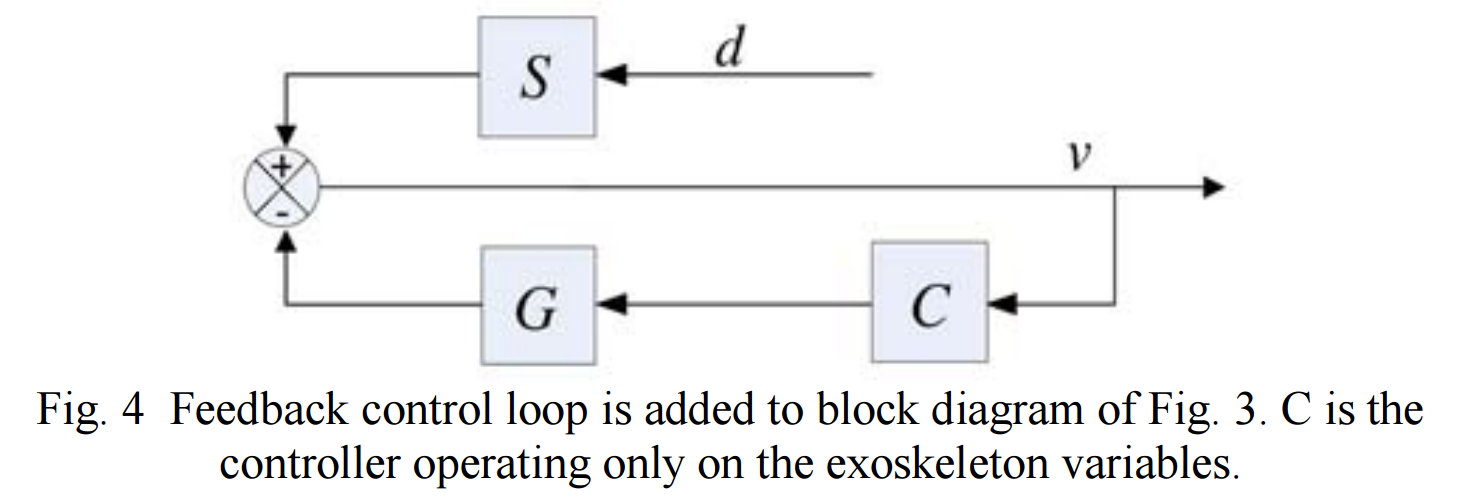
\includegraphics[width=4.0in]{exos/figs/bleex_control_diag_2.png}
\end{figure}

As a note, positive feedback is normally avoided in control design because it amplifies disturbances.  In the case of BLEEX, designers sacrifice disturbance rejection to maximize the response of the suit to its wearer.  Users must therefore take action to stabilize and balance out disturbances.

\begin{figure}[ht]
  \centering
  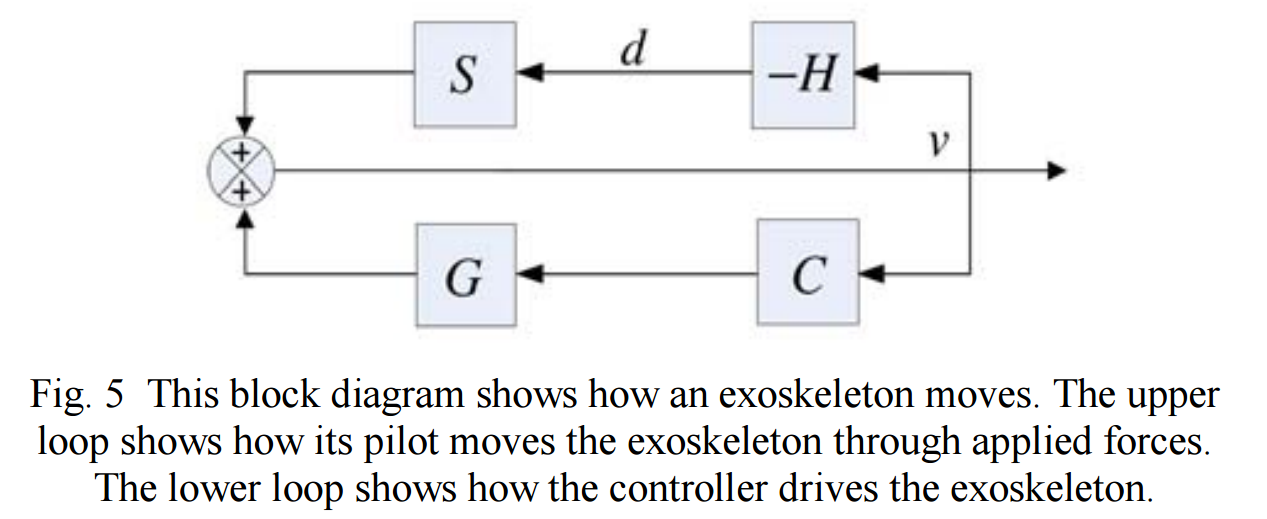
\includegraphics[width=4.0in]{exos/figs/bleex_control_diag_3.png}
\end{figure}

For sensing, BLEEX uses information from \textbf{8 encoders} and \textbf{16 accelerometers} to determine angle, angular velocity, and angular acceleration of eight actuated joints. It includes a \textbf{foot switch and load distribution sensor} at each foot. Eight single axis \textbf{force sensors} provide measurements required to perform low level force control at each actuator. An \textbf{inclinometer} indicates the orientation of the backpack relative to gravity. Using this sensitivity amplification control scheme, BLEEX has achieved successful walking at 1.3 m/s with a 34kg payload \cite{sesitivityAmpPaper2005}.

\subsection{Assessment and Recommendations}

Sensitivity amplification is a current best-in-class control strategy.  The exoskeleton shadows the user and uses exoskeleton data for joint angle, velocity, and acceleration and the exoskeleton model to minimize torques experienced by the human torque.  The process and hardware are relatively simple yet effective.   However, the approach has several significant disadvantages including heavy reliance on an accurate exoskeleton model and the fact that sensitivity amplification will amplify disturbances.  Note that in combat situations this latter point is critical as a sensitivity amplification will amplify forces acting on the suit and the operator will have to re-act to compensate.  The only way to compensate for or resist external forces in this setting is to filter them out, which would be extremely challenging unless additional sensory equipment is provided.  As one possibility, a sensitivity optimization approach may be paired with sEMG data to estimate user intent and provide such a filter.  Note this type of implementation would present its own challenges considering limitations in sensing and calibration of current EMG systems. 


\bibliographystyle{plain}
\bibliography{exos/bleex}

The figures in this section were obtained from \cite{sesitivityAmpPaper2005}. Materials presented are based on the references above.


\section{HAL}
\label{exo:hal}
\begin{refsection}[exos/hal.bib]

% keywords: model-based control; predefined gait trajectory; strength augmentation; rehabilitation.\\

The hybrid assistive limb (HAL) exoskeleton is developed by the University of Tsukuba and Cyberdyne for human strength augmentation and as an assistive gait device in rehabilitation.  Although several prototypes have been developed, this section focuses on the most recent HAL-5 model (specifically the non-clinical type, HAL-5 Type-B). Though HAL-5 is a full body exoskeleton, only hip, knee joints, and ankle are actuated in the sagittal plane.  The exoskeleton uses DC motors with harmonic drives at hip, knee, ankle joints (in some models the ankle joints act as passive springs).  HAL weighs 23kg and includes an on-board AC100V battery as the power source, which is designed to support maximum velocity human walking and standing torque requirements.  The battery allows for 160 min of continuous operation and enables the exoskeleton to lift up to 70kg \cite{HALassist2011}.  

Human operators attach to HAL at the waist with a belt, and at the calf and thigh using harnesses. HAL's frame does not transfer load to the ground.  Instead, HAL adjusts hip, knee and ankle torques to amplify its operator's torque. The exoskelton's sensory system includes bioelectric sensing (including \textbf{sEMG}), \textbf{angular sensors}, \textbf{acceleration sensors}, and \textbf{center of pressure / center of gravity} (COP/COG) sensors.  COP/COG sensing is provided through shoes with ground reaction force sensors.  The joint measurements are provided by potentiometers.
In at least one version of HAL the bioelectric data comes from sEMG sensors installed below the operator's hip and above the knee (on both front and back).
An IMU installed in HAL's backpack is used to estimate torso pose.


\begin{figure}[ht]
  \centering
  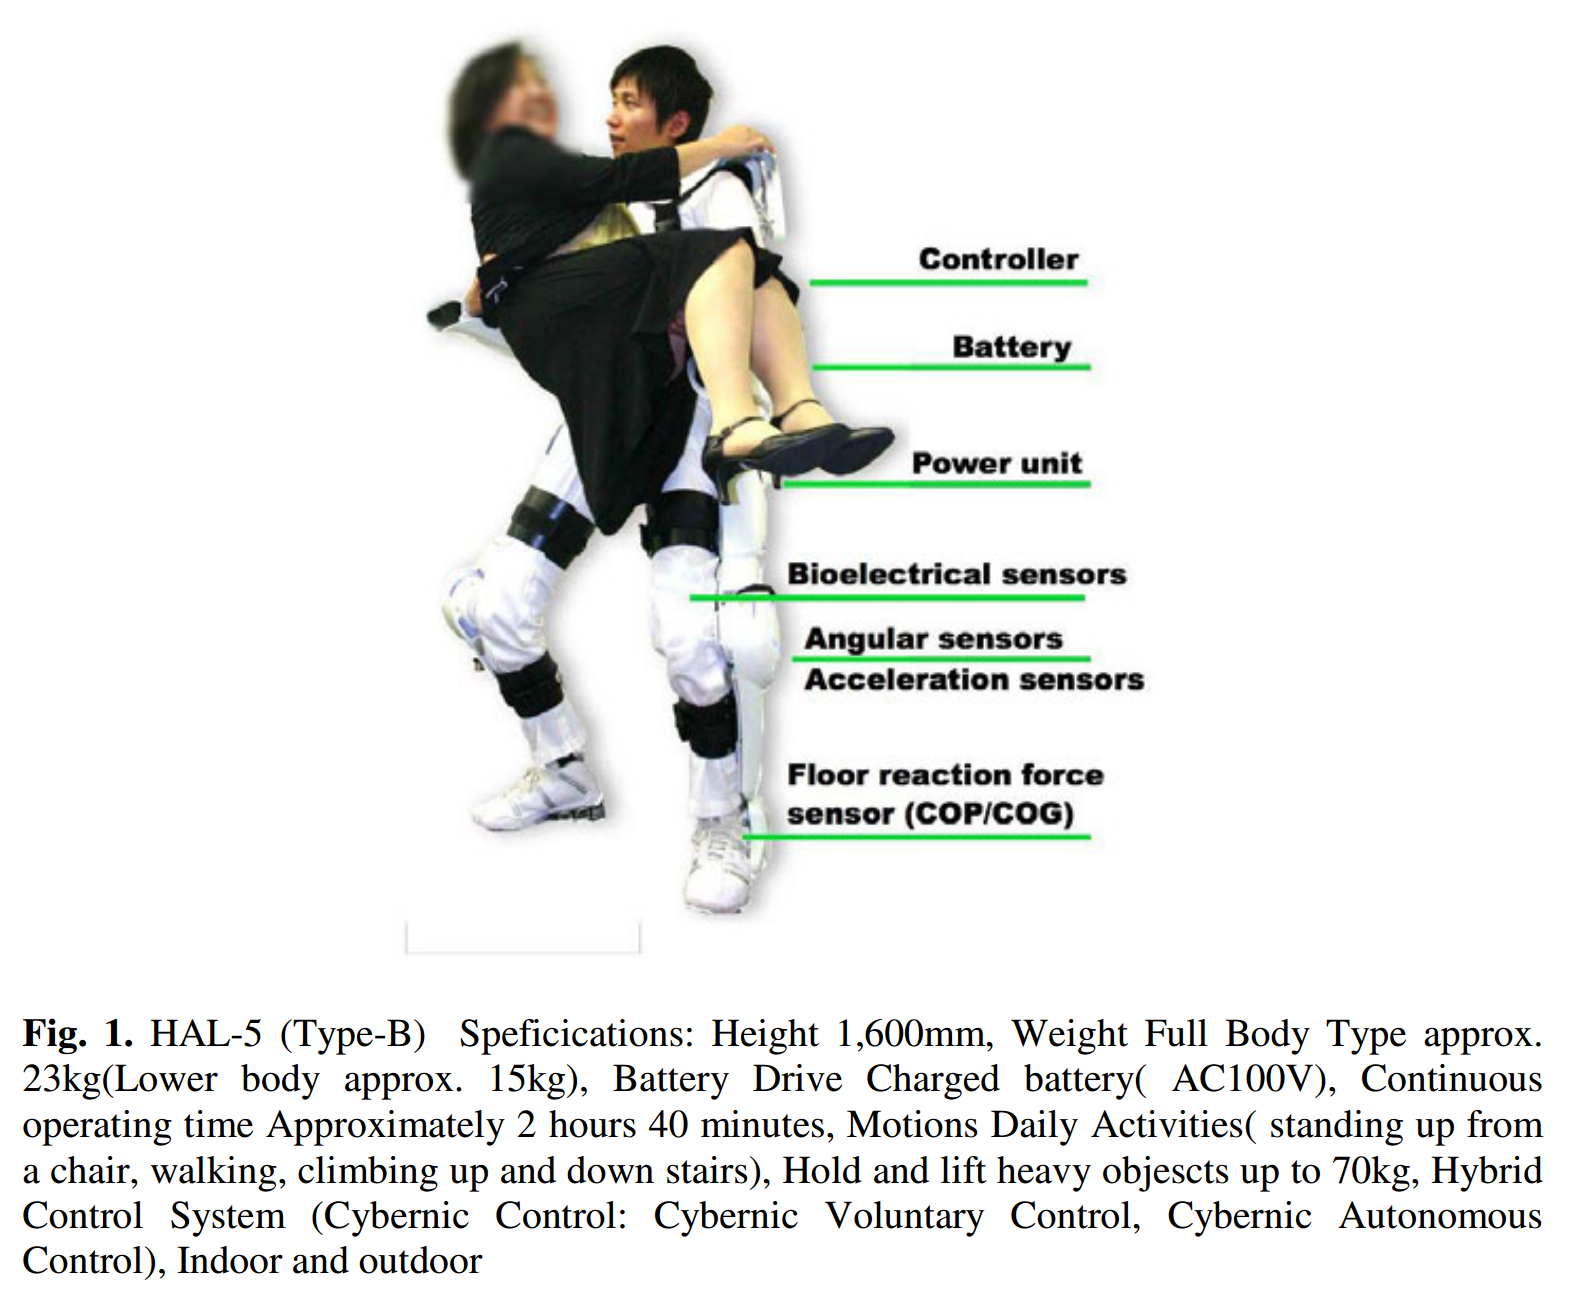
\includegraphics[width=3.5in]{exos/figs/hal-5_B_diagram.png}
\end{figure}


\subsubsection{Control}

HAL has two types of control systems designed for different application domains.  For gait assistance and rehabilitation, HAL uses an autonomous control system that carries the user through predefined gait trajectories by controlling knee and hip joints (the ankles behave as passive springs).  Gait phase intention is estimated from COP/COG sensors.  The exoskeleton drives the wearer to follow pre-recorded desired joint patterns.

The second control strategy, a model-based approach for human strength augmentation, estimates human intention from sEMG activity and provides power to augment torque provided by the operator.  A relatively autonomous torque assist strategy in \cite{HALmodelControlKnee2010} recognizes user intention to take a step by thresholding sEMG data.  The approach provides a knee torque response including an assitive torque component, a viscous damping component that reduces high velocity motion for safety, and a gravity compensation torque.  
%In \cite{HALvTorqueImp2002}, HAL uses myoelectric data to estimate muscle torque based on the difference between flexor and extensor muscle activities.  

In \cite{HALmuscleImped2005}, an impedance control strategy controls the viscoelastic properties of HAL's knee joint from a musculoskeletal model of operator's limb moving in concert with the exoskeleton.  The controller uses sEMG sensor data to estimate muscle torque based on the difference between flexor and extensor muscle activities.  The authors note the sEMG model requires significant calibration effort.  
Viscoelastic torques are computed according to
\[\tau_{a,i} = \alpha_i(-D_i \theta_i - K_i \theta_i),\]  
based on a variable gain set by $\alpha_i$.  The net knee actuator torque is
\[\tau_i = \tau_{a,i} + \tau_\mu + \tau_c .\]
The torque includes a $\tau_c$ term compensating for mechanical (actuator) impedance and $\tau_\mu$, a scaled version of the human torque (as estimated  from sEMG data).  The $K_i$ and $D_i$ terms in $\tau_{a,i}$ are viscoelastic parameters (based on the operator's muscles) in the human-exoskeleton model.  These parameters are estimated on-line using a weighted least-squares method.  In this case, the angular velocity data required for the impedance controller is estimated from a state observer.

%
\begin{figure}[ht]
  \centering
  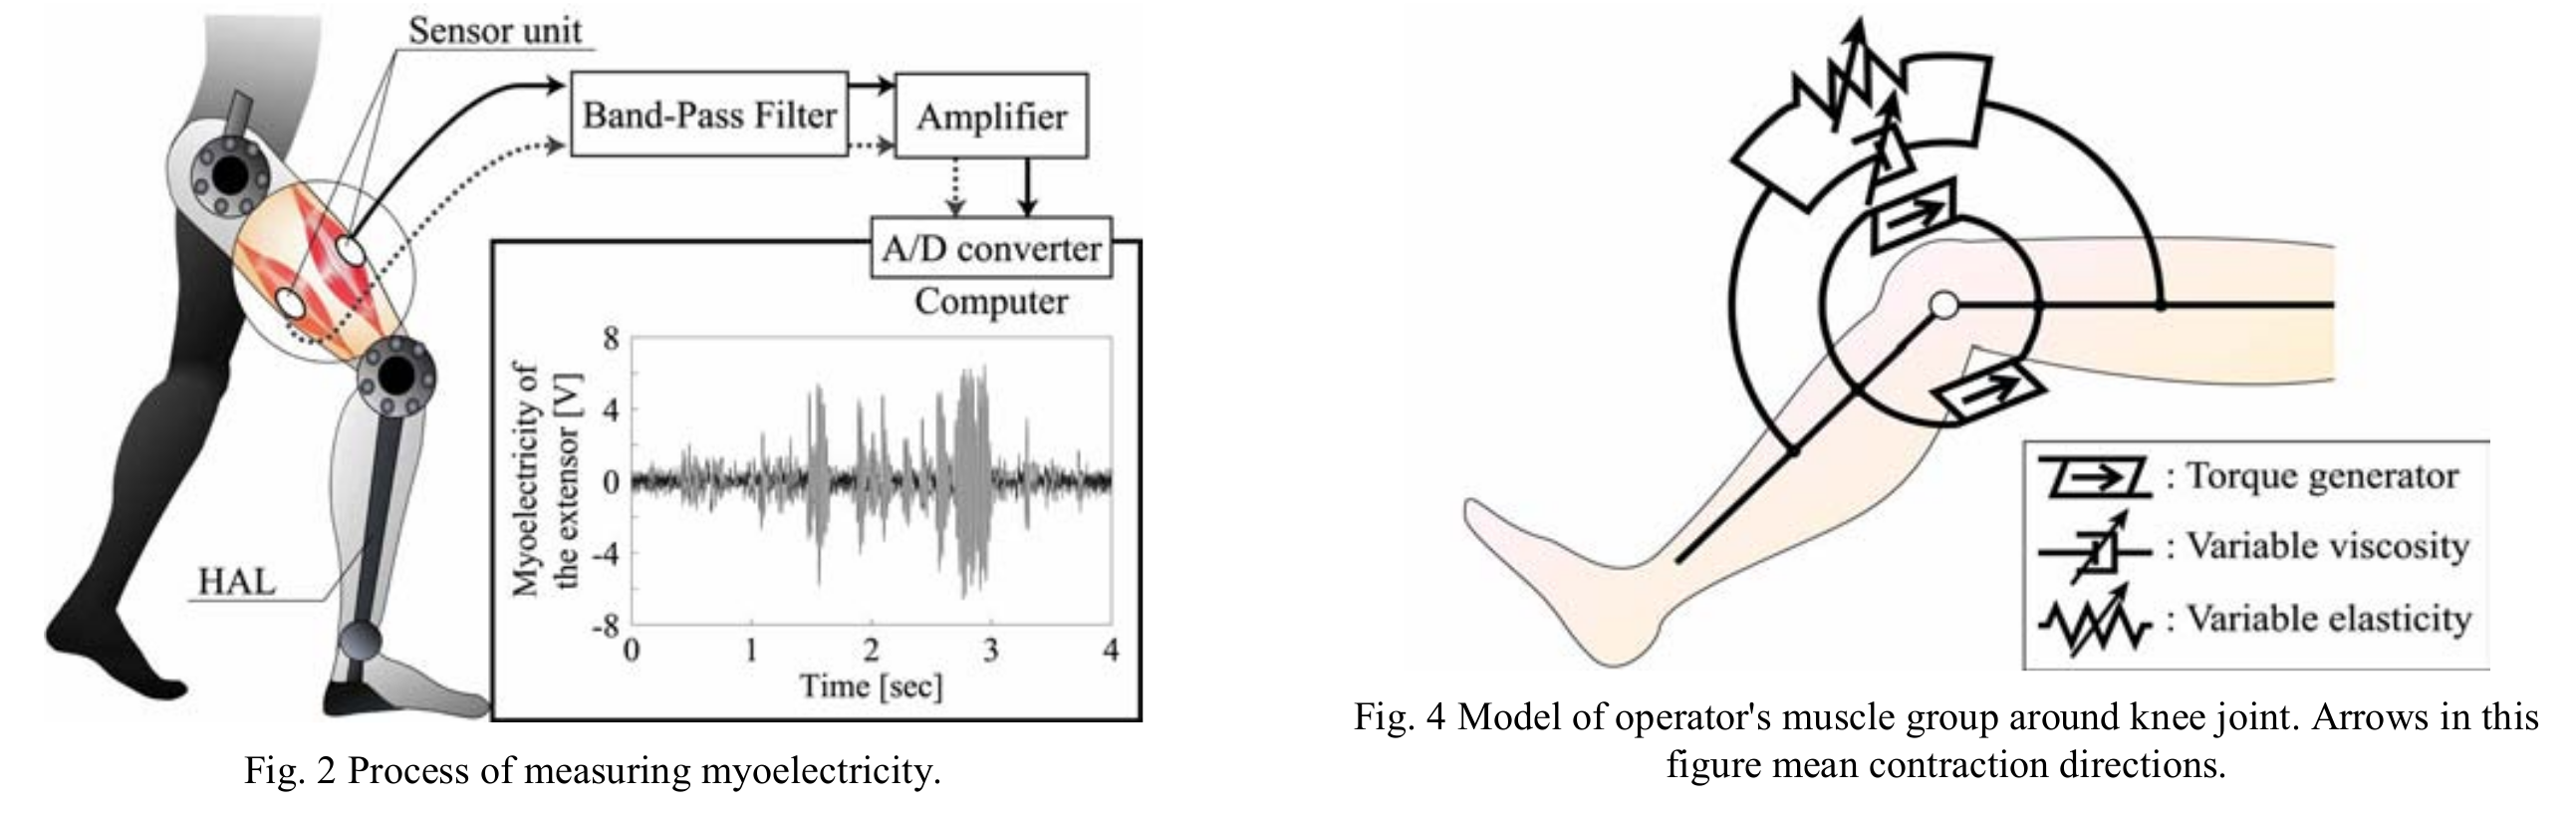
\includegraphics[width=6in]{exos/figs/hal_viscoelastic_control.png}
\end{figure}
%
%

While experiments in \cite{HALmuscleImped2005} only consider leg swing-up and swing-down, a similar control approach in \cite{HALvTorqueImp2002} switches the dynamics based controller to compensate for swing and stance phases in walking gait.  In this case, the gait transitions are detected by thresholding foot sensors and required angular velocity (and acceleration) data are determined by numerically differentiating angular encoders.


\subsection{Assessment and Recommendations}

Compared to sensitivity amplification methods, HAL's use of EMG data allows it to estimate intention without amplifying external disturbances.  While direct sensing of user intention is ideal for noisy, contract-rich environments, sEMG data is extremely difficult to work with due to high filtering and calibration requirements.  A hybrid strategy which uses sensitivity amplification and sEMG data (possibly thresholded) to filter user intention could prove effective.  Additionally, Section~\ref{survey:recommend} mentions new capabilities in nano-fabrication and MEMs technologies that have produced new high-density, wearable sensing arrays. These and similarly advanced sensing technology may facilitate direct measurement of interaction forces (i.e. estimating pressure / force and exoskeleton contact locations), which could potentially filter external disturbances from user generated input to estimate intent.

\nocite{*}
\printbibliography[heading=subbibliography]

The figures in this section were obtained from \cite{HALmuscleImped2005,HALassist2011}.  Materials presented are based on the references above.

\end{refsection}




%%% Local Variables:
%%% mode: latex
%%% TeX-master: "../survey"
%%% End:


\section{XoR}
\label{exo:XoR}
\begin{refsection}[exos/xor.bib]

keywords: model-based control; strength augmentation; hybrid actuation; pneumatic actuation; electric motors;\\

\begin{figure}[ht]
  \centering
  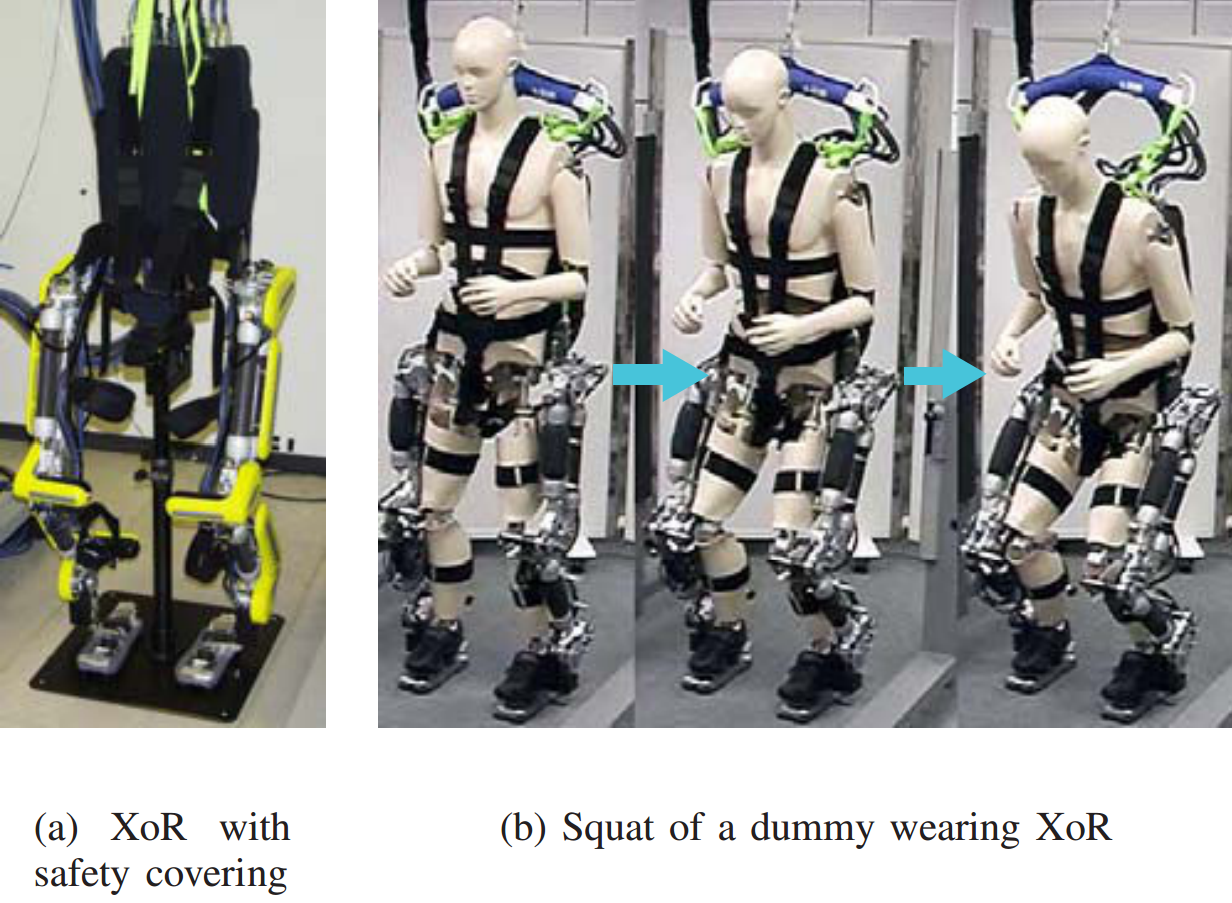
\includegraphics[width=4.0in]{exos/figs/xor.png}
\end{figure}

The XoR is a prototype, light-weight lower-body exoskeleton that uses a hybrid pneumatic-electric drive system that \textbf{reduces weight} while providing \textbf{precise torque control}, \textbf{backdrivability}, and a \textbf{desirable force / velocity} profile.  The exoskeleton is designed to serve in rehabilitation settings to augment operators' strength and assist with postural control for persons with disabilities.

\begin{figure}[ht]
  \centering
  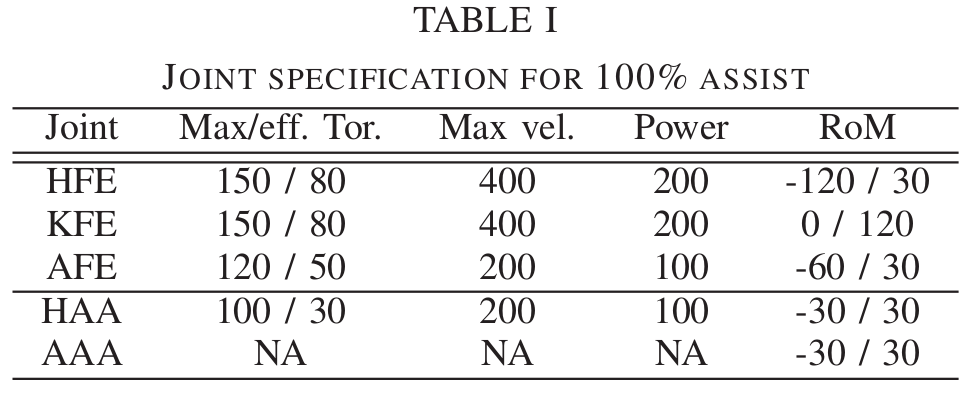
\includegraphics[width=3.5in]{exos/figs/xor_joint_rom.png}
\end{figure}

The XoR weighs 30kg and includes 10 DOF with 6 active joints (flexion / extension of hip, knee, and ankles) and 6 passive (hip abduction/adduction joints, hip rotation, and ankle adduction/abduction).  The active joints are powered by hybrid actuators comprised of an \emph{air muscle} and an electric motor.  The hybrid actuation scheme uses a unilateral air muscle layout to compensate for gravity and bilateral electric motors with relatively small gear ratio (57.5) to serve as the dynamic compensator.

The actuation scheme is complementary in that the electric motors have a quick response time and produce high peak torque for short amounts of time, while air muscles have a delayed response (true of pneumatic systems in general due to the compressibility of air) with better power density and sustained torque.  The hybrid drive system sums the two to develop a desired torque profile that achieves the benefits of both and reduces weight and motor size.  The system offers high torque control with negligable stick-slip and backdrivability.

\begin{figure}[ht]
  \centering
  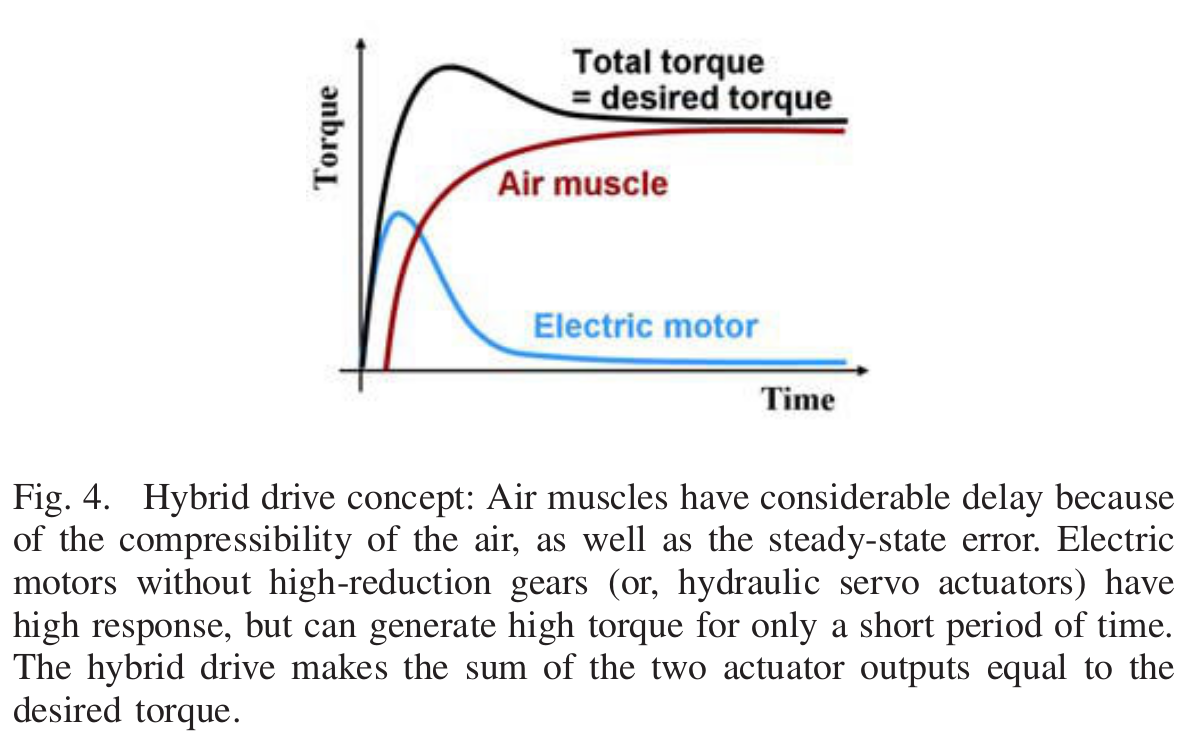
\includegraphics[width=3.5in]{exos/figs/xor_hybrid_drive_torque_time.png}
\end{figure}  

A challenge in using air muscles is that force reduces quadratically as a function of contraction.  For instance, at 30\% contraction, the force produced by FESTO rubber air muscles vanishes.  To address the issue, XoR is strategically places air muscles to generate forces in desired configurations.  

\begin{figure}[ht]
  \centering
  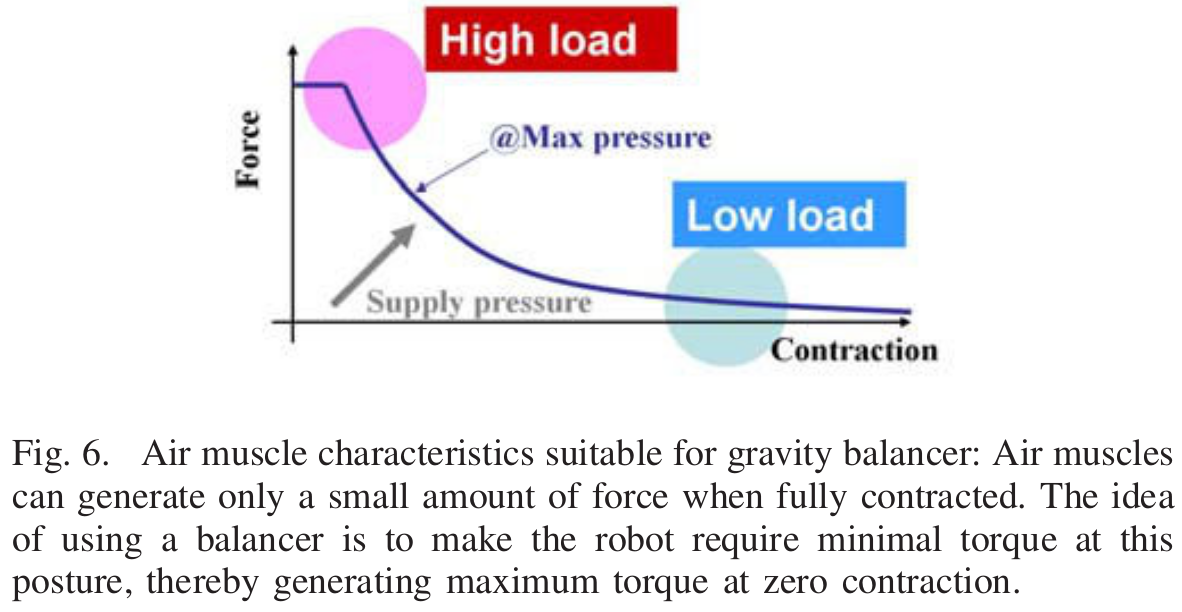
\includegraphics[width=3.5in]{exos/figs/xor_air_muscle_force_vs_contraction.png}
\end{figure}

In implementation, the XoR uses rubber air muscles (MDSP-40) connected to pulleys via tendons and to EP regulators in the backpack (a constant pressure and cam system is being tested to reduce weight required for backpack air valves).  The electric actuator is a geared, 200W brushless DC motor (Maxon EC powermax 30) rated at 4.7 A, which transmits power to joints through a belt and pulley system with a 57.5 gear ratio. the motor's 0.12 Nm output torque provides up to 34.5 Nm (for short duration) at every joint and is backdrivable.  The design yields a relatively high range of motion (up to 120 degrees) with a load capacity 150 Nm.  However, experiments reveal the need for bi-directional pneumatic actuation at hip joints.

For sensing, XoR is equipped with rotary encoders at joints, an IMU in the backpack, load cells in the feet, and is networked to servers capable of providing EMG, NIRS, and EEG data.  A control PC running at 1 KHz, pulse counter, amplifiers, Digital IO are external and so not included in the weight of the unit.  Human operators are outfitted with a goniometer.


\subsubsection{Control}

The XoR control strategy applied in \cite{XoRkinemExtraction2012} has two main components.  First, a proportional-derivative (PD) feedback controller tracks desired joint angles and angular velocities that correspond to the state of the exoskeleton required to assist the human operator.  To obtain this state (specifying the desired joint angles / velocities), the controller simultaneously measures the joint angle trajectories of the human user (goniometer) and of the robot (encoders), and uses canonical correlation analysis (CCA) to extract latent variables in the kinematic relationship between the two.

\begin{figure}[ht]
  \centering
  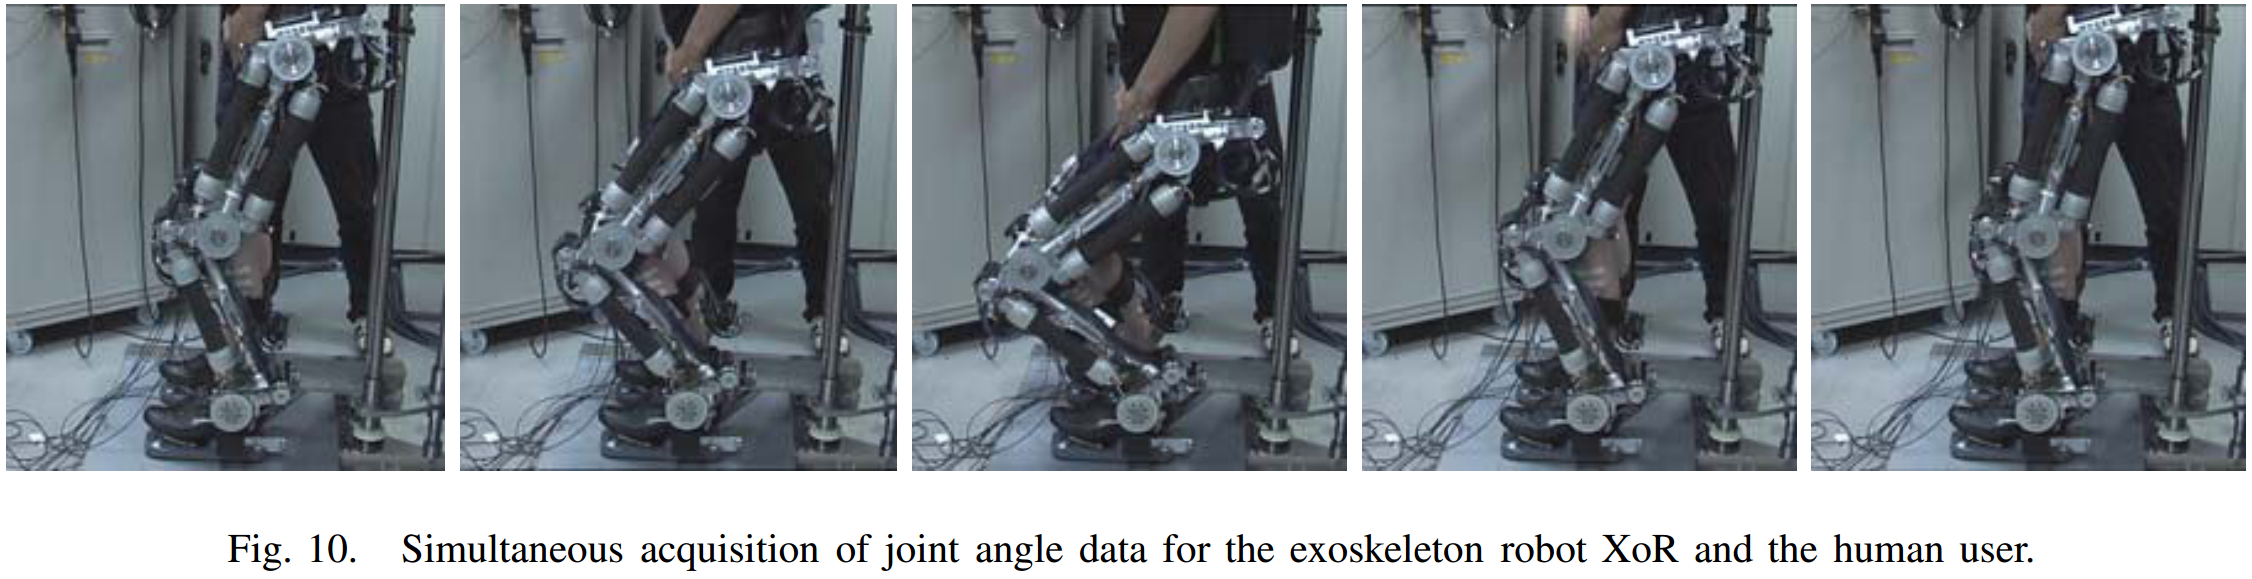
\includegraphics[width=6.0in]{exos/figs/xor_joint_angles.png}
\end{figure}

To avoid relying on high gain feedback, XoR incorporates user intent through EMG data.  The controller rectifies and low pass filters (10 Hz cut-off) data measured in the pilot's quadriceps femoris, tensor fasciae latate, gluteus medius, and tibialis anterior. 
It sets desired joint angles and velocities, ${\bf x} = ({\bf \theta} \dot{\bf \theta})$, from the EMG data, ${\bf u} = (EMG_1 \cdot EMG_n)$, using a linear prediction model, 
\[{\bf x}(k+1) = \mA{\bf x}(k)+\mB{\bf u}(k),\].  
The controller uses the angular measurements required to perform CCA and EMG data to derive the model's $\mA$ and $\mB$ terms.  The predicted state from EMG model provides the desired input to yet another PD controller: 
\[\tau_i = K_p (\theta_i^d - \theta_i) + K_d (\dot\theta_i^d - \dot \theta_i),\] 
with gains of $K_p = 1000$ and $K_d = 100$.

In hip tracking experiments, the team found EMG data to be helpful.  When using EMG signals, XoR achieved a mean squared error of $1.8E^{-3}$.  Without the EMG data, the mean squared error increased to $2.1$.  Additional experiments confirm the air muscles can effectively perform gravity compensation when used in conjunction with electric actuators (to correct for torque errors induced by inaccuracies in the model mapping position to toque in air muscles).


\subsection{Assessment and Recommendations}

The XoR prototype uses a promising hybrid actuation scheme to achieve both fast peak torque response and higher sustained torque while remaining lightweight.  They track human motion with feedback from a goniometer and feedforward control provided by EMG data.  These human intention / sensing modalities are both difficult to implement due to noise and calibration issues.  However, capturing the user intent is important, especially in the presence of external disturbances.  If the sensory system were improved (e.g, wearable ``robot skin'' sensing arrays), this exoskeleton design could be highly effective. 

\nocite{*}
\printbibliography[heading=subbibliography]

The figures in this section were obtained from \cite{xorDesign2011,XoRkinemExtraction2012}. Materials presented are based on the references above.

\end{refsection}

% \subsection{EXO-UL7}
\label{exo:exo-ul7}

keywords: model-based control; strength augmentation;\\

\begin{figure}[ht]
  \centering
  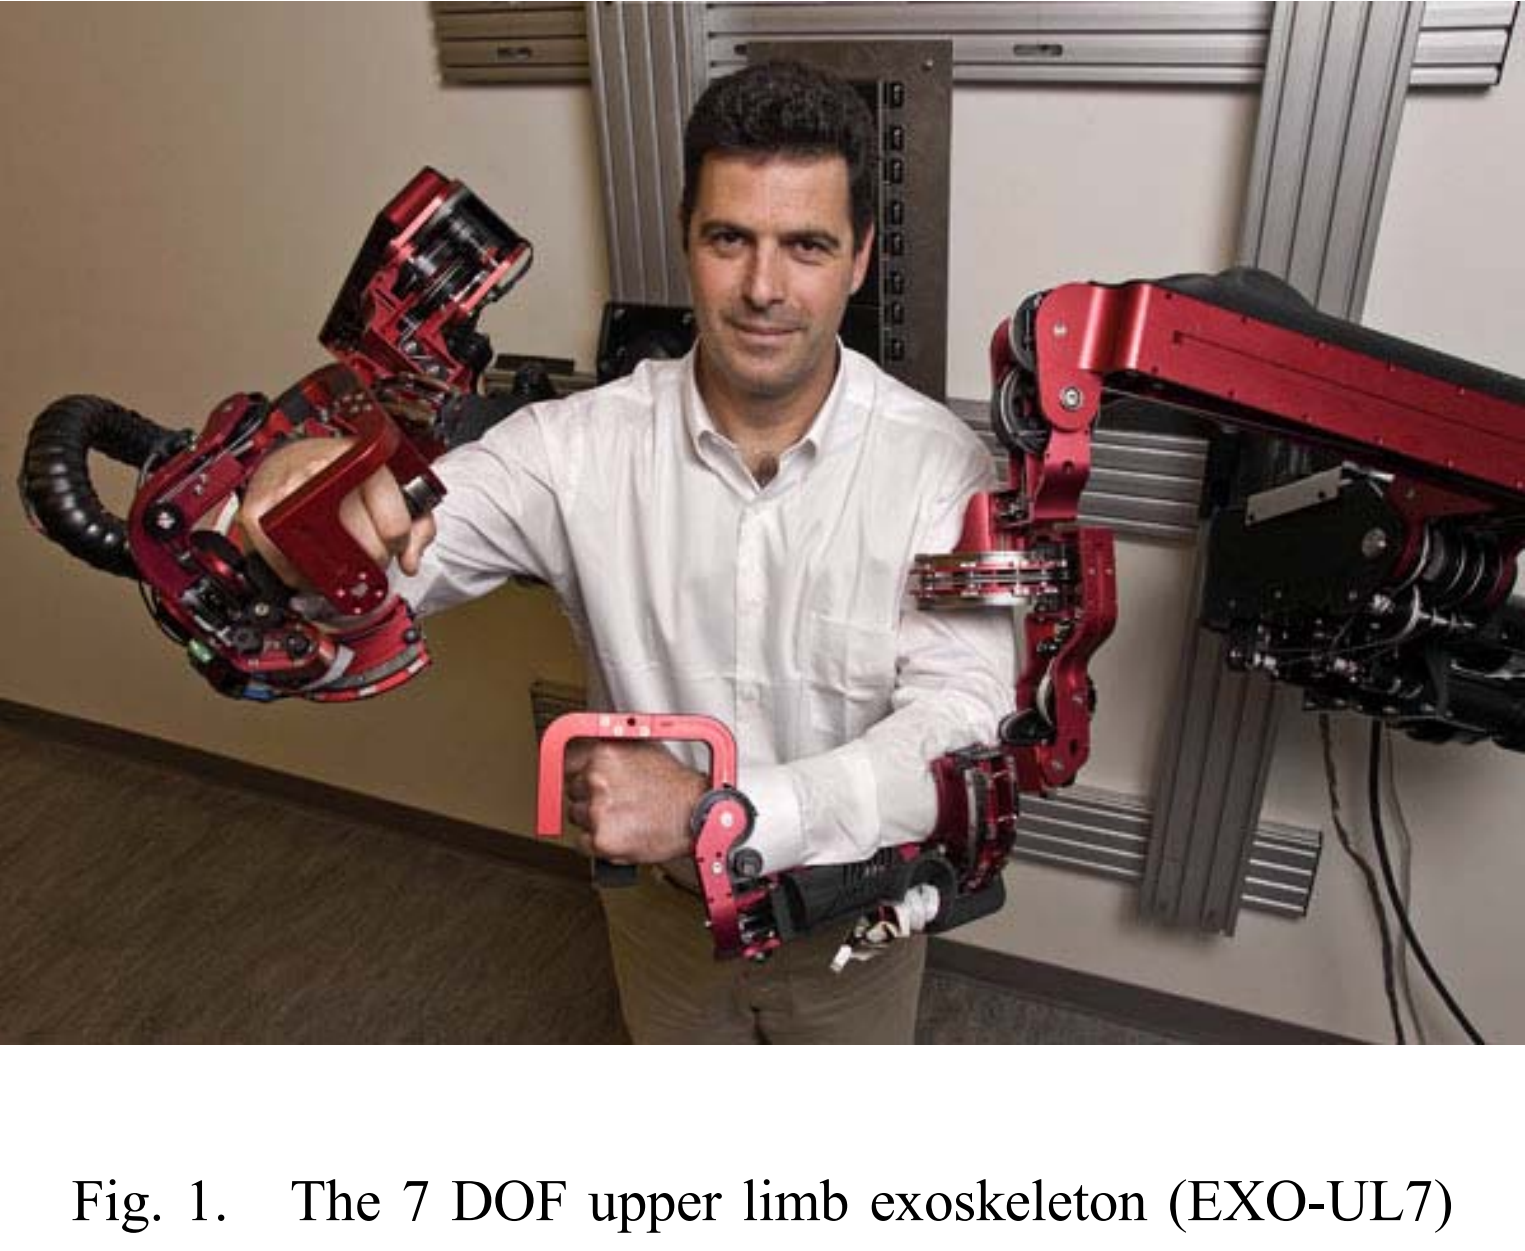
\includegraphics[width=4.0in]{exos/figs/exo-ul7.png}
\end{figure}


Although this study focuses on lower-body exoskeltons, we include the EXO-UL7 7 DOF upper-extremity exoskeleton for its novel actuation scheme and principled design. 

-------------------------------------------------

(Called CADEN - "cable driven dexterous exoskeleton for neurorehabilitation" in [[EXOul7design]])

Design:

7 DOF model; cable-actuated; proximal motor placement and distal cable-pulley reductions for low inertia, high stiffness links with backdrivable transmissions with zero backlash.  "Enables full glenohumeral, elbow, and wrist joint functionality." -- [[EXOul7design]]

% set the Human Machine Interface (HMI) at the neuromuscular level ... as one of the primary command signals... Use sEMG signals.  -- http://bionics.seas.ucla.edu/research/exoskeleton_device_3.html

[[EXOul7design]] contains data from a dynamic / kinematic study of human motion during everyday tasks in order to determine design requirements for exo.

3 lvls of safety mechanisms: 1) built in mechanical -- phys. stops, 2) electrical -- three wearer e-stops including an observer e-stop, an enable button which must be held, and a foot switch e-stop, and 3) software -- redundant position sensing (pots, Midori, Fullerton; shaft encoder, HP), one at either side of power train, monitor both joint motion and motor position. -- [[EXOul7design]]

Control bandwidth -- targeted 10Hz based on achievable frequency range of human arm which is btwn 2Hz and 5Hz.  They found shoulder joint had 1st resonant mode at 6 Hz. -- [[EXOul7design]]

Weight: 3.5 and 6kg from links 1 and links 2-7 (resp.). -- [[EXOul7design]]

Articulation: 7 single axis revolute joints.  Use three pulleys (90 and 180 deg configurations) at joints to keep cable length constant. Stack of pulleys required -- two pulleys representing agonist muscle groups and two for antagonist -- [[EXOul7design]]

Singularities: Design movable joint mechanisms that allow adjustment of singularity within 15deg based on user preferences. -- [[EXOul7design]]

Power transmission: shafts, cables, fluid lines, and gear trains.  Use pulleys for speed reductions and backdrivability.  2-stage pulleys in proximal joints 1-4 and single stage for more distal (5-7). -- [[EXOul7design]]

Motors for joints 1–4 were mounted on the stationary base, achieving a 60% reduction in overall weight of the moving parts. The remaining three motors, whose torque requirements are substantially less, were positioned on the forearm -- [[EXOul7design]]


Control Strategy:

Model-based control -- "proposed HMI takes advantage of the electro-chemical-mechanical delay, which inherently exists in the musculoskeletal system, between the time when the neural system activates the muscular system and the time when the muscles generate moments around the joints. The myoprocessor is a model of the human muscle running in real-time and in parallel to the physiological muscle.   During the electro-chemical-mechanical time delay, the system will gather information regarding the physiological muscle’s neural activation level based on processed sEMG signals, the joint position, and angular velocity, and will predict using the myoprocessor the force that will be generated by the muscle before physiological contraction occurs. By the time the human muscles contract, the exoskeleton will move with the human in a synergistic fashion, allowing natural control of the exoskeleton as an extension of the operator's body." %-- http://bionics.seas.ucla.edu/research/exoskeleton_device_3.html

Say they use neuro control strategy to avoid having to trigger motion based on human movement / force (required in position, force-impedance control) -- [[EXOul7design]]


References:

Cavallaro E., J. Rosen, J. C. Perry, S. Burns, B. Hannaford, Hill Based Model as a Myoprocessor for a Neural Controlled Powered Exoskeleton Arm – Parameter Optimization, Proceedings of the 2005 IEEE international Conference on Robotics and Automation, ICRA 2005, pp. 4525 – 4530, Barcelona Spain, April 2005

Rosen J,, J. C. Perry, N. Manning, S. Burns, B. Hannaford, The Human Arm Kinematics and Dynamics During Daily Activities – Toward a 7 DOF Upper Limb Powered Exoskeleton, - ICAR 2005 – Seattle WA, July 2005. [ CP19]

Perry J.C., J. Rosen, Design of a 7 Degree-of-Freedom Upper-Limb Powered Exoskeleton Proceedings of the 2006 BioRob Conference, Pisa, Italy, February, 2006.

Cavallaro E., J. Rosen, J. C. Perry, S. Burns, Myoprocessor for Neural Controlled Powered Exoskeleton Arm, IEEE Transactions on Biomedical Engineering, pp. 2387-2396, Vol. 53, No. 11, November 2006

Perry J. C., J. Rosen, S. Burns, Upper-Limb Powered Exoskeleton Design, IEEE Transactions on Mechatronics, Volume 12, No. 4, pp. 408-417, August 2007 <<EXOul7design>>

Rosen J., and J.C. Perry, Upper Limb Powered Exoskeleton, Journal of Humanoid Robotics, Vol. 4, No. 3 (2007) 1–20

Miller, L.M. and J. Rosen, 2010." Comparison of multi-sensor admittance control in joint space and task space for a seven degree of freedom upper
limb exoskeleton," 3rd IEEE RAS and EMBS International Conference on Biomedical Robotics and Biomechatronics (BioRob). <<EXOul7admitJointTaskCmp>>

Wen, Y., J. Rosen, and L. Xiaoou, 2011." PID admittance control for an upper limb exoskeleton," American Control Conference (ACC).  <<EXOul7admit>>

-------------------------------------------------

\subsection{Assessment and Recommendations}

The EXO-UL7 is a well-designed upper body exosekelton that is experimenting with new sEMG based control mechanisms.  The control approach is not as refined and needs to be developed further before field applications due to reliance on sEMG data.  
% As mentioned in Sections~\ref{exo:bleex} and \ref{exo:hal}, there are advantages to .


The figures in this section were obtained from \cite{EXOul7design2007,EXOul7pidAdmit2011}.  Materials presented are based on the references above.


\section{Discussion}

Discussion to be written.

\section{Conclusions and Recommendations}

Conclusions and Recommendations to be written.

% \bibliographystyle{plain}
% \bibliography{exo}

\end{document}
